\chapter{Plan de Trabajo}
	\label{chap:work}
	
	\section{Resultados y Productos Esperados}
	
	Esta secci\'{o}n abarca los resultados del entrenamiento de la red y el
an\'{a}lisis estad\'{i}stico posterior a esto. Junto a lo anterior, se listan
los productos que se esperan producir como parte del desarrollo de la
investigaci\'{o}n.
	
Resultados esperados comprenden:
	\begin{itemize}
	  \item Encontrar un modelo de red neuronal que permita mejorar los tiempos
	  empleados por los veh\'{i}culos y que se reduzcan los congestionamientos por
	  causa de su mala administraci\'{o}n.
	  \item Que la toma de decisiones de forma distribuida por parte de los
	  sem\'{a}foros logre evitar tiempos de espera innecesarios. 
	  \item Reducci\'{o}n de los errores cometidos por la red de forma que para
	  otro trabajo de investigaci\'{o}n pueda ser puesto a prueba en lugares como
	  Heredia, Alajuela y Cartago.
	  \item Lograr un margen de error aceptable el cual permita en un futuro pasar
	  a la implementaci\'{o}n en ambiente real de la red neuronal.
	\end{itemize}

Se espera producir:
	\begin{itemize}
	  \item Programa de simulaci\'{o}n para entrenamiento de la red.
	  \item Implementaci\'{o}n del algoritmo de programaci\'{o}n de la red.
	  \item An\'{a}lisis estad\'{i}stico donde se demuestre el desempe\~{n}o
	  logrado por la red, y se contraste con los valores que se presentan actualmente por
	  el sistema de control de tr\'{a}fico del MOPT.\\
	\end{itemize}
	
	
	
	\section{Riesgos del proyecto}
	
	\begin{table}[!h]
			\centering
			\begin{tabular}{|p{1.3cm}|p{3cm}|p{1cm}|p{1.6cm}|p{1.8cm}|p{6cm}|}
				\hline
				\textbf{ID} & \textbf{Riesgo} & \textbf{Prob.} & \textbf{Impacto} & \textbf{Magnitud} & \textbf{Acciones de
				Administraci\'{o}n}\\ \hline 				
				RNN-1 & No contar con los datos estad\'{i}scos generados por el sistema de
				control de tr\'{a}fico del MOPT necesarios para contrastar los resultados
				generados por la red neuronal & 2 & 4 & 8 & Mantener contacto activo con
				el miembro del centro de control de tr\'{a}fico de forma que no se pierda
				la colaboraci\'{o}n mediante llamadas, correos o visitas al centro. En caso
				de materializarse se proceder\'{a} a realizar los datos estad\'{i}stico de
				forma manual.\\ 
				\hline 
				RNN-2 & No lograr obtener un modelo de red neuronal que funcione de forma
				adecuada de acuerdo con las expectativas de la tesis. & 2 & 4 & 8 &
				Investigaci\'{o}n constante de alternativas que permitan obtener el
				modelo de red esperado. De igual forma se realizar\'{a}n evaluaciones
				constantes (luego de cada prueba de entrenamiento) con el fin de mantener un
				registro controlado de los resultados que se vayan obteniendo. 
				\\ 
				\hline 						
				RNN-3 & No contar con los factores necesarios para probar el correcto
				funcionamiento de la red neuronal causando una falta de pruebas del
				desempe\~{n}o de la misma & 2 & 3 & 6 & Revisar de forma exhaustiva la lista
				de factores obtenida de los trabajos anteriores, y validarla de forma que se
				garantice una correcta selecci\'{o}n de los escenarios para pruebas.
				\\
				\hline	
				 
			\end{tabular}
			\caption{Riesgos}
			\label{tab:risk}
		\end{table}
		
	\section{Proyecci\'{o}n o cronograma}	
	\begin{figure}[htp]
 		\centering
 		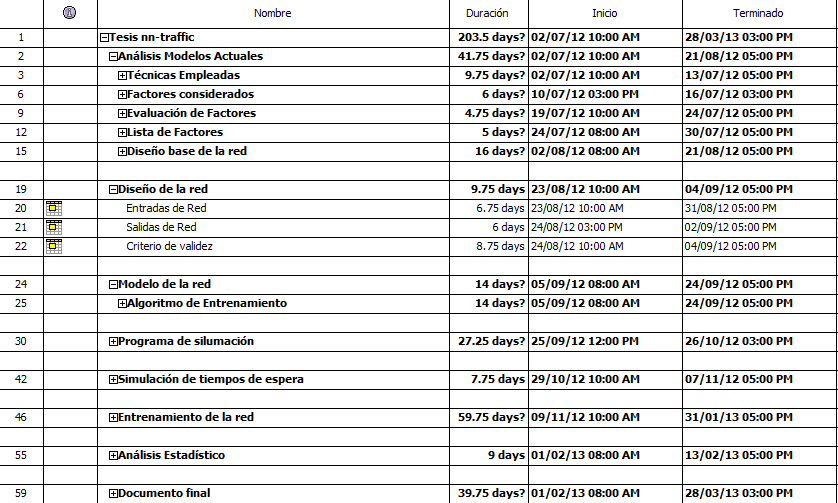
\includegraphics[width=1.1\textwidth,
 		height=0.65\textheight]{images/cronoMIN.png}
 		\caption{Cronograma}
 		\label{fig:Crono}
 	\end{figure}
	
	\begin{landscape}
	\begin{figure}[htp]
 		\centering 		
 		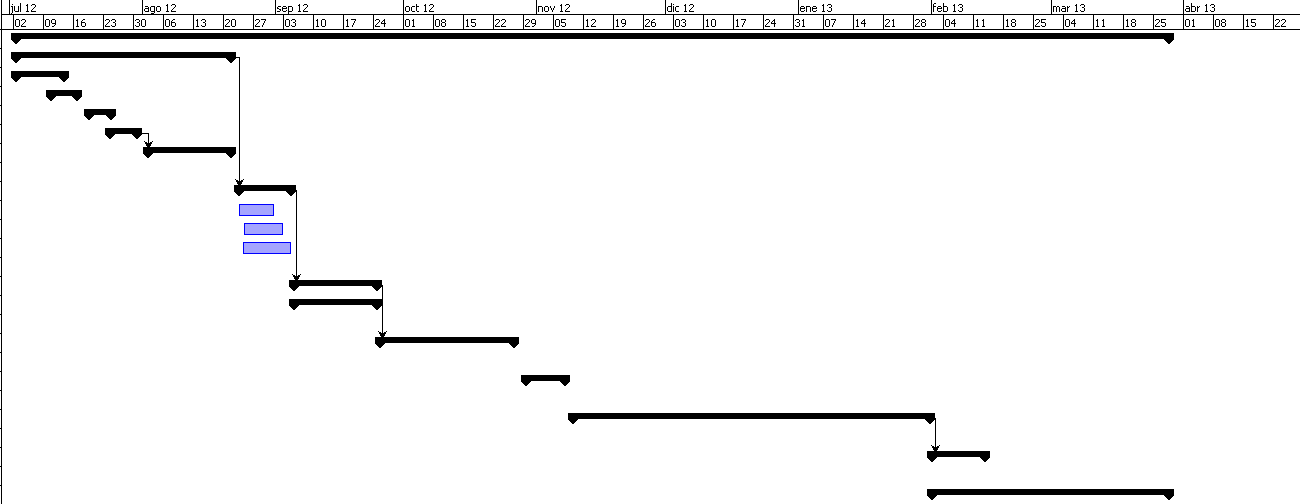
\includegraphics[width=20cm,height=15cm]{images/ganttMIN2.png}
 		\caption{Diagrama de Gantt}
 		\label{fig:gantt}
 	\end{figure}
	\end{landscape}
	
	\sectionbreak